% Graphic for TeX using PGF
% Title: /home/ben/workspace/devs-ex-machina/paper/pqueue.dia
% Creator: Dia v0.97.3
% CreationDate: Wed Nov 25 18:04:10 2015
% For: ben
% \usepackage{tikz}
% The following commands are not supported in PSTricks at present
% We define them conditionally, so when they are implemented,
% this pgf file will use them.

\ifx\du\undefined
  \newlength{\du}
\fi
\setlength{\du}{15\unitlength}
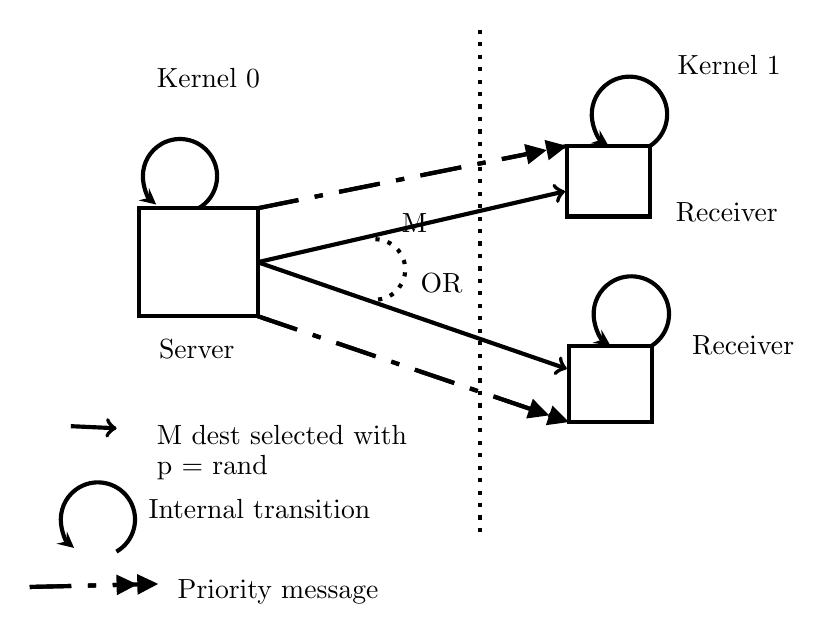
\begin{tikzpicture}
\pgftransformxscale{1.000000}
\pgftransformyscale{-1.000000}
\definecolor{dialinecolor}{rgb}{0.000000, 0.000000, 0.000000}
\pgfsetstrokecolor{dialinecolor}
\definecolor{dialinecolor}{rgb}{1.000000, 1.000000, 1.000000}
\pgfsetfillcolor{dialinecolor}
\pgfsetlinewidth{0.100000\du}
\pgfsetdash{}{0pt}
\pgfsetdash{}{0pt}
\pgfsetmiterjoin
\definecolor{dialinecolor}{rgb}{1.000000, 1.000000, 1.000000}
\pgfsetfillcolor{dialinecolor}
\fill (5.000000\du,5.150000\du)--(5.000000\du,7.750000\du)--(7.850000\du,7.750000\du)--(7.850000\du,5.150000\du)--cycle;
\definecolor{dialinecolor}{rgb}{0.000000, 0.000000, 0.000000}
\pgfsetstrokecolor{dialinecolor}
\draw (5.000000\du,5.150000\du)--(5.000000\du,7.750000\du)--(7.850000\du,7.750000\du)--(7.850000\du,5.150000\du)--cycle;
\pgfsetlinewidth{0.100000\du}
\pgfsetdash{}{0pt}
\pgfsetdash{}{0pt}
\pgfsetbuttcap
{
\definecolor{dialinecolor}{rgb}{0.000000, 0.000000, 0.000000}
\pgfsetfillcolor{dialinecolor}
% was here!!!
\pgfsetarrowsend{to}
\definecolor{dialinecolor}{rgb}{0.000000, 0.000000, 0.000000}
\pgfsetstrokecolor{dialinecolor}
\draw (7.850000\du,6.450000\du)--(15.250970\du,4.742084\du);
}
\pgfsetlinewidth{0.100000\du}
\pgfsetdash{}{0pt}
\pgfsetdash{}{0pt}
\pgfsetbuttcap
{
\definecolor{dialinecolor}{rgb}{0.000000, 0.000000, 0.000000}
\pgfsetfillcolor{dialinecolor}
% was here!!!
\pgfsetarrowsend{to}
\definecolor{dialinecolor}{rgb}{0.000000, 0.000000, 0.000000}
\pgfsetstrokecolor{dialinecolor}
\draw (7.850000\du,6.450000\du)--(15.295050\du,9.017863\du);
}
\pgfsetlinewidth{0.100000\du}
\pgfsetdash{}{0pt}
\pgfsetdash{}{0pt}
\pgfsetmiterjoin
\definecolor{dialinecolor}{rgb}{1.000000, 1.000000, 1.000000}
\pgfsetfillcolor{dialinecolor}
\fill (15.300000\du,3.650000\du)--(15.300000\du,5.350000\du)--(17.300000\du,5.350000\du)--(17.300000\du,3.650000\du)--cycle;
\definecolor{dialinecolor}{rgb}{0.000000, 0.000000, 0.000000}
\pgfsetstrokecolor{dialinecolor}
\draw (15.300000\du,3.650000\du)--(15.300000\du,5.350000\du)--(17.300000\du,5.350000\du)--(17.300000\du,3.650000\du)--cycle;
\pgfsetlinewidth{0.100000\du}
\pgfsetdash{}{0pt}
\pgfsetdash{}{0pt}
\pgfsetmiterjoin
\definecolor{dialinecolor}{rgb}{1.000000, 1.000000, 1.000000}
\pgfsetfillcolor{dialinecolor}
\fill (15.345000\du,8.460000\du)--(15.345000\du,10.300000\du)--(17.345000\du,10.300000\du)--(17.345000\du,8.460000\du)--cycle;
\definecolor{dialinecolor}{rgb}{0.000000, 0.000000, 0.000000}
\pgfsetstrokecolor{dialinecolor}
\draw (15.345000\du,8.460000\du)--(15.345000\du,10.300000\du)--(17.345000\du,10.300000\du)--(17.345000\du,8.460000\du)--cycle;
\pgfsetlinewidth{0.100000\du}
\pgfsetdash{{1.000000\du}{0.400000\du}{0.200000\du}{0.400000\du}}{0cm}
\pgfsetdash{{1.000000\du}{0.400000\du}{0.200000\du}{0.400000\du}}{0cm}
\pgfsetbuttcap
{
\definecolor{dialinecolor}{rgb}{0.000000, 0.000000, 0.000000}
\pgfsetfillcolor{dialinecolor}
% was here!!!
\definecolor{dialinecolor}{rgb}{0.000000, 0.000000, 0.000000}
\pgfsetstrokecolor{dialinecolor}
\draw (7.850000\du,7.750000\du)--(15.345000\du,10.300000\du);
}
\definecolor{dialinecolor}{rgb}{0.000000, 0.000000, 0.000000}
\pgfsetstrokecolor{dialinecolor}
\draw (7.850000\du,7.750000\du)--(14.398293\du,9.977905\du);
\pgfsetmiterjoin
\definecolor{dialinecolor}{rgb}{0.000000, 0.000000, 0.000000}
\pgfsetfillcolor{dialinecolor}
\fill (14.791123\du,10.375629\du)--(15.345000\du,10.300000\du)--(14.952170\du,9.902276\du)--cycle;
\pgfsetmiterjoin
\definecolor{dialinecolor}{rgb}{0.000000, 0.000000, 0.000000}
\pgfsetfillcolor{dialinecolor}
\fill (14.317769\du,10.214582\du)--(14.871646\du,10.138952\du)--(14.478817\du,9.741228\du)--cycle;
\pgfsetlinewidth{0.100000\du}
\pgfsetdash{{1.000000\du}{0.400000\du}{0.200000\du}{0.400000\du}}{0cm}
\pgfsetdash{{1.000000\du}{0.400000\du}{0.200000\du}{0.400000\du}}{0cm}
\pgfsetbuttcap
{
\definecolor{dialinecolor}{rgb}{0.000000, 0.000000, 0.000000}
\pgfsetfillcolor{dialinecolor}
% was here!!!
\definecolor{dialinecolor}{rgb}{0.000000, 0.000000, 0.000000}
\pgfsetstrokecolor{dialinecolor}
\draw (7.850000\du,5.150000\du)--(15.300000\du,3.650000\du);
}
\definecolor{dialinecolor}{rgb}{0.000000, 0.000000, 0.000000}
\pgfsetstrokecolor{dialinecolor}
\draw (7.850000\du,5.150000\du)--(14.319673\du,3.847381\du);
\pgfsetmiterjoin
\definecolor{dialinecolor}{rgb}{0.000000, 0.000000, 0.000000}
\pgfsetfillcolor{dialinecolor}
\fill (14.859182\du,3.993772\du)--(15.300000\du,3.650000\du)--(14.760491\du,3.503609\du)--cycle;
\pgfsetmiterjoin
\definecolor{dialinecolor}{rgb}{0.000000, 0.000000, 0.000000}
\pgfsetfillcolor{dialinecolor}
\fill (14.369019\du,4.092463\du)--(14.809837\du,3.748691\du)--(14.270328\du,3.602300\du)--cycle;
% setfont left to latex
\definecolor{dialinecolor}{rgb}{0.000000, 0.000000, 0.000000}
\pgfsetstrokecolor{dialinecolor}
\node[anchor=west] at (17.650000\du,5.250000\du){Receiver};
% setfont left to latex
\definecolor{dialinecolor}{rgb}{0.000000, 0.000000, 0.000000}
\pgfsetstrokecolor{dialinecolor}
\node[anchor=west] at (5.200000\du,8.550000\du){Server};
% setfont left to latex
\definecolor{dialinecolor}{rgb}{0.000000, 0.000000, 0.000000}
\pgfsetstrokecolor{dialinecolor}
\node[anchor=west] at (5.650000\du,14.400000\du){Priority message};
\pgfsetlinewidth{0.100000\du}
\pgfsetdash{}{0pt}
\pgfsetdash{}{0pt}
\pgfsetbuttcap
{
\definecolor{dialinecolor}{rgb}{0.000000, 0.000000, 0.000000}
\pgfsetfillcolor{dialinecolor}
% was here!!!
\pgfsetarrowsend{stealth}
\definecolor{dialinecolor}{rgb}{0.000000, 0.000000, 0.000000}
\pgfsetstrokecolor{dialinecolor}
\pgfpathmoveto{\pgfpoint{17.299933\du}{3.650044\du}}
\pgfpatharc{57}{-236}{0.908447\du and 0.908447\du}
\pgfusepath{stroke}
}
% setfont left to latex
\definecolor{dialinecolor}{rgb}{0.000000, 0.000000, 0.000000}
\pgfsetstrokecolor{dialinecolor}
\node[anchor=west] at (4.950000\du,12.400000\du){Internal transition};
% setfont left to latex
\definecolor{dialinecolor}{rgb}{0.000000, 0.000000, 0.000000}
\pgfsetstrokecolor{dialinecolor}
\node[anchor=west] at (11.050000\du,5.500000\du){M};
% setfont left to latex
\definecolor{dialinecolor}{rgb}{0.000000, 0.000000, 0.000000}
\pgfsetstrokecolor{dialinecolor}
\node[anchor=west] at (5.150000\du,10.600000\du){M dest selected with};
% setfont left to latex
\definecolor{dialinecolor}{rgb}{0.000000, 0.000000, 0.000000}
\pgfsetstrokecolor{dialinecolor}
\node[anchor=west] at (5.150000\du,11.400000\du){p = rand};
\pgfsetlinewidth{0.100000\du}
\pgfsetdash{{\pgflinewidth}{0.200000\du}}{0cm}
\pgfsetdash{{\pgflinewidth}{0.200000\du}}{0cm}
\pgfsetbuttcap
{
\definecolor{dialinecolor}{rgb}{0.000000, 0.000000, 0.000000}
\pgfsetfillcolor{dialinecolor}
% was here!!!
\definecolor{dialinecolor}{rgb}{0.000000, 0.000000, 0.000000}
\pgfsetstrokecolor{dialinecolor}
\draw (13.200000\du,0.850000\du)--(13.200000\du,13.150000\du);
}
% setfont left to latex
\definecolor{dialinecolor}{rgb}{0.000000, 0.000000, 0.000000}
\pgfsetstrokecolor{dialinecolor}
\node[anchor=west] at (5.150000\du,2.000000\du){Kernel 0};
% setfont left to latex
\definecolor{dialinecolor}{rgb}{0.000000, 0.000000, 0.000000}
\pgfsetstrokecolor{dialinecolor}
\node[anchor=west] at (17.695000\du,1.705000\du){Kernel 1};
% setfont left to latex
\definecolor{dialinecolor}{rgb}{0.000000, 0.000000, 0.000000}
\pgfsetstrokecolor{dialinecolor}
\node[anchor=west] at (18.900000\du,1.200000\du){};
% setfont left to latex
\definecolor{dialinecolor}{rgb}{0.000000, 0.000000, 0.000000}
\pgfsetstrokecolor{dialinecolor}
\node[anchor=west] at (19.550000\du,2.850000\du){};
% setfont left to latex
\definecolor{dialinecolor}{rgb}{0.000000, 0.000000, 0.000000}
\pgfsetstrokecolor{dialinecolor}
\node[anchor=west] at (18.045000\du,8.455000\du){Receiver};
\pgfsetlinewidth{0.100000\du}
\pgfsetdash{}{0pt}
\pgfsetdash{}{0pt}
\pgfsetbuttcap
{
\definecolor{dialinecolor}{rgb}{0.000000, 0.000000, 0.000000}
\pgfsetfillcolor{dialinecolor}
% was here!!!
\pgfsetarrowsend{stealth}
\definecolor{dialinecolor}{rgb}{0.000000, 0.000000, 0.000000}
\pgfsetstrokecolor{dialinecolor}
\pgfpathmoveto{\pgfpoint{17.344933\du}{8.460044\du}}
\pgfpatharc{57}{-236}{0.908447\du and 0.908447\du}
\pgfusepath{stroke}
}
\pgfsetlinewidth{0.100000\du}
\pgfsetdash{}{0pt}
\pgfsetdash{}{0pt}
\pgfsetbuttcap
{
\definecolor{dialinecolor}{rgb}{0.000000, 0.000000, 0.000000}
\pgfsetfillcolor{dialinecolor}
% was here!!!
\pgfsetarrowsend{stealth}
\definecolor{dialinecolor}{rgb}{0.000000, 0.000000, 0.000000}
\pgfsetstrokecolor{dialinecolor}
\pgfpathmoveto{\pgfpoint{6.424932\du}{5.150040\du}}
\pgfpatharc{60}{-230}{0.894049\du and 0.894049\du}
\pgfusepath{stroke}
}
\pgfsetlinewidth{0.100000\du}
\pgfsetdash{{\pgflinewidth}{0.200000\du}}{0cm}
\pgfsetdash{{\pgflinewidth}{0.200000\du}}{0cm}
\pgfsetbuttcap
{
\definecolor{dialinecolor}{rgb}{0.000000, 0.000000, 0.000000}
\pgfsetfillcolor{dialinecolor}
% was here!!!
\definecolor{dialinecolor}{rgb}{0.000000, 0.000000, 0.000000}
\pgfsetstrokecolor{dialinecolor}
\pgfpathmoveto{\pgfpoint{10.749941\du}{7.350007\du}}
\pgfpatharc{84}{-95}{0.728943\du and 0.728943\du}
\pgfusepath{stroke}
}
% setfont left to latex
\definecolor{dialinecolor}{rgb}{0.000000, 0.000000, 0.000000}
\pgfsetstrokecolor{dialinecolor}
\node[anchor=west] at (11.500000\du,6.950000\du){OR};
\pgfsetlinewidth{0.100000\du}
\pgfsetdash{}{0pt}
\pgfsetdash{}{0pt}
\pgfsetbuttcap
{
\definecolor{dialinecolor}{rgb}{0.000000, 0.000000, 0.000000}
\pgfsetfillcolor{dialinecolor}
% was here!!!
\pgfsetarrowsend{stealth}
\definecolor{dialinecolor}{rgb}{0.000000, 0.000000, 0.000000}
\pgfsetstrokecolor{dialinecolor}
\pgfpathmoveto{\pgfpoint{4.447461\du}{13.421630\du}}
\pgfpatharc{60}{-230}{0.894049\du and 0.894049\du}
\pgfusepath{stroke}
}
\pgfsetlinewidth{0.100000\du}
\pgfsetdash{}{0pt}
\pgfsetdash{}{0pt}
\pgfsetbuttcap
{
\definecolor{dialinecolor}{rgb}{0.000000, 0.000000, 0.000000}
\pgfsetfillcolor{dialinecolor}
% was here!!!
\pgfsetarrowsend{to}
\definecolor{dialinecolor}{rgb}{0.000000, 0.000000, 0.000000}
\pgfsetstrokecolor{dialinecolor}
\draw (3.350000\du,10.400000\du)--(4.450000\du,10.450000\du);
}
\pgfsetlinewidth{0.100000\du}
\pgfsetdash{{1.000000\du}{0.400000\du}{0.200000\du}{0.400000\du}}{0cm}
\pgfsetdash{{1.000000\du}{0.400000\du}{0.200000\du}{0.400000\du}}{0cm}
\pgfsetbuttcap
{
\definecolor{dialinecolor}{rgb}{0.000000, 0.000000, 0.000000}
\pgfsetfillcolor{dialinecolor}
% was here!!!
\definecolor{dialinecolor}{rgb}{0.000000, 0.000000, 0.000000}
\pgfsetstrokecolor{dialinecolor}
\draw (2.358440\du,14.273440\du)--(5.450000\du,14.200000\du);
}
\definecolor{dialinecolor}{rgb}{0.000000, 0.000000, 0.000000}
\pgfsetstrokecolor{dialinecolor}
\draw (2.358440\du,14.273440\du)--(4.450282\du,14.223748\du);
\pgfsetmiterjoin
\definecolor{dialinecolor}{rgb}{0.000000, 0.000000, 0.000000}
\pgfsetfillcolor{dialinecolor}
\fill (4.956078\du,14.461804\du)--(5.450000\du,14.200000\du)--(4.944204\du,13.961945\du)--cycle;
\pgfsetmiterjoin
\definecolor{dialinecolor}{rgb}{0.000000, 0.000000, 0.000000}
\pgfsetfillcolor{dialinecolor}
\fill (4.456219\du,14.473678\du)--(4.950141\du,14.211874\du)--(4.444345\du,13.973819\du)--cycle;
\end{tikzpicture}
